\Chapter{Tervezés és implementáció}

% TODO: Keras áttekintése.

% TODO: Szakaszonként bemutatni a jellemző kinyerés implementációját.

% TODO: Részletesen, osztálydiagrammal bemutatni a konvolúciós hálós osztályozáshoz készített program szerkezetét.

Ebben a fejezetbe egy képminősítési problémát szeretnék megoldni, ahol a célunk az lesz, hogy megállapítsuk, melyik osztályba tartozik a bemeneti kép. Ahhoz, hogy ezt megvalósítsuk, szükségünk van sok (minnél különböző annál jobb) bemeneti képekre a tanítás során. A konvolúciós neurális hálózat (CNN) képzésével és a neurális hálózat (NN) megtanulásával meg lehet jósolni, hogy melyik osztályba tartozik a kép.

A legfontosabb dolog, hogy megértsük, hogy a ezek a modellek bármilyen típusú osztályra kiképezhetjük, ha egy osztályba tartozó bemeneti képekre tanítjuk be a hálózatunkat, akkor tesztelésnél pontosan felismeri ezeket az osztályokat, viszont kevésbbé ismeri fel a más osztályba tartozó képeket. Figyelembe kell venni a bemeneti képeket, hiszen általuk tanul a hálózat.

\section{Keras}

Az implementálás részhez a Keras deep learing könyvtárat használtam a pythonban. A könyvtár segítségével egyszerűen lehet létrezhozni a konvolúciós neurális hálózatot (CNN).

\begin{figure}[h]
\centering

\includegraphics[scale=0.5]{images/keras}
\caption{A \textit{Keras} szoftvercsomag logója}
\label{fig:k}
\end{figure}

A Keras egy magas szintű neurális hálózat API, Python-ban írva, ami a TensorFlow, CNTK és a Theano felett fut. (\Aref{fig:k}. ábrán látható a logója.) A Keras a gyors kísérletezésre összpontosít. A kód általában rövid, letisztult és jól szervezett.

A Keras deep learning könyvtár a továbbiakra érdemes használni:

\begin{itemize}
\item Lehetővé teszi az egyszerű és gyors prototípus készítését (a felhasználóbarátság, a modularitás és a bővíthetőség révén).
\item Támogatja mind a konvolúciós hálózatokat, mind a visszatérő hálózatokat, mind a kettő kombinációit.
\item A CPU és a GPU zökkenőmentesen működik.
\end{itemize}


\section{Adathalmaz}

Mielőtt belevágnánk a modell kiépítésébe, szükségünk van tanító és teszt adatkészletre. Az kínai karakter adatbázisokat 2 csoportra oszthatjuk: online vagy offline. \Aref{fig:offline_online} ábrán látható pár példa.
\begin{itemize}
\item Online: Az online adatgyűjtés egy speciális digitális tollal (Anoto) történik. Lehetséges nyomtatott sablonok vagy szabadkezes írás. Az írás során az online adatok (stroke pályagörbéje: (x, y) koordináták szekvenciái) kerülnek rögzítésre az Anoto tollal, majd ezeket később a számítógépekre továbbítják.
\item Offline: Az offline adatgyűjtés érdekében a kézzel írt oldalakat szkennelnek be (300 dpi felbontásban), hogy színes képeket kapjanak. Az annotációs eszközök segítségével a képeket szegmentálni és címkézni kell. Az annotáció után az adatbázisok hátterének 255 a pixel értéke előtéri képpontok értéke 0-254 közötti (szürke árnyalatos). Tehát bináris képeket úgy kaphatunk, ha egyszerűen megváltoztatjuk az előtér pixelét 1-re és a háttér-pixeleket 0-ra.
\end{itemize}

\begin{figure}[h]
\centering
\captionsetup{justification=centering}
\begin{tabular}{ l r }
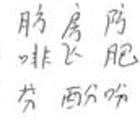
\includegraphics[scale=1.2]{images/offlineChars} & 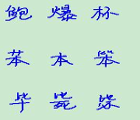
\includegraphics[scale=1.2]{images/onlineChars}
\end{tabular}
\caption{Offline és online karakterek
\hspace{\textwidth}Forrás:\url{http://www.nlpr.ia.ac.cn/databases/handwriting/Online_database.html}}
\label{fig:offline_online}
\end{figure}

\subsection{CASIA} 

A CASIA adatbázisok hat online és hat offline adathalmazból. Mindegyik adatbázis esetében három elszigetelt karakterkészlet és három kézzel írt szöveg tartozik. Mind az online, mind az offline esetekben az elszigetelt karakterek adatkészletei körülbelül 3,9 millió 7,356 osztályból (7,185 kínai karakter és 171 szimbólum) tartalmaznak, a kézzel írt szövegek pedig mintegy 5,090 oldalas és 1,35 millió karakteres mintát tartalmaznak. Az összes adatot szegmentálták és annotálták a karakterek szintjén és minden adatkészletet szabványos képzési és tesztalkalmazásokra osztottak fel.

\subsection{HITMWDB}

A HITMWDB adabázist összehasonlítva a korábbi kéziratos adatbázisokkal, ebben az adatbázisban legalább három különbség van. Először is, a kézírás természetes módon íródott és nincsenek vonalzók, amelyek segítségével a szöveget egyenes vonalban lehet létrehozni. Másodszor, a kézi másolás alapjául szolgáló szövegeket szisztematikus módon mintavételezik és az írókat gondosan választják ki. Harmadszor, az adatok levél vagy közvetítő által lett összegyűjtve, ami valódi kézírási jelenségeket eredményez, például a rosszírás és a javítás.\\

A tanító és a teszt adatbázis aránya általában 8:2 (tanító:tesztelő). Az arány megfelelő kiválasztása fontos. Két egymással versengő probléma van: kevesebb képzési adatokkal, a paraméterbecslések nagyobb eltérést mutatnak. Kevesebb tesztelési adat mellett a teljesítménystatisztikája nagyobb lesz. Elmondható, hogy olyan megosztására kell törekedni, ahol a variancia nem túl magas.

\section{Implementáció}

\subsection{Konvolúciós hálózat felépítése}

A konvolúciós neurális hálózat kiépítésének folyamata mindig négy nagy lépést foglal magában.

\begin{enumerate}
\item Konvolúció
\item Pooling
\item RELU
\item Teljesen összekapcsolt réteg
\end{enumerate}

\subsection{Csomagok}

Először importáljuk a szükséges keras csomagokat, amelyek segítségével a konvolúciós hálózatunkat kiépítjük. Meg kell győződni arról, hogy minden csomagot megfelelően telepítettünk a gépünkbe. A csomagok telepítését a \textit{pip} vagy az \textit{anaconda} csomag menedzserrel hajtható végre.

\begin{python}
# A Keras konyvtarak es csomagok importalasa
from keras.layers import Sequential, Conv2D, MaxPooling2D, Dense, Flatten
from keras.layers.normalization import BatchNormalization
from keras.layers import Activation, Input
from keras import models
\end{python}

A Sequential-t a keras.models-ből importáltuk, hogy inicializáljuk a neurális hálózat modelljét. A neurális hálózatnak két alapvető módja lehet: réteges vagy diagrammos.

A keras.layers-ből importáltunk Conv2D-t, ez a CNN első lépésének végrehajtása a képzési képeken. Mivel itt képekkel dolgozunk, amelyek alapvetően 2 dimenziós tömbök, ezért a Convolution2D-t használjuk. A Convolution-D-t a videók kezelése során lehet használni, ahol a harmadik dimenzió lesz az idő.

A keras.layer-ből importáltunk MaxPooling2D-t, amelyet a művelet összevonására használunk, ami a CNN létrehozásának folyamata. Az adott neurális hálózat kiépítéséhez Maxpooling funkciót használunk, léteznek különböző típusú poolozási műveletek, mint a Min Pooling, a Mean Pooling stb. Itt a MaxPooling-ban szükségünk van a legmagasabb érték pixelre az adott érdeklődési területről.

A Flatten-t a keras.layers-ből importáltunk, amelyet a Flattening-hez használunk. Az átlapolás az a folyamat, amely során az összes kapott kétdimenziós tömböt egy hosszú, folyamatos lineáris vektorba konvertáljuk.

A keras.layer-ből importáltunk Dense-t, amely a neuronhálózat teljes összekapcsolására szolgál, ami a negyedik lépés a CNN létrehozásának folyamatában.

\subsection{Rétegek}

Most létrehozunk egy objektumot a Sequential osztályból:

\begin{python}
classifier = Sequential()
\end{python}

Most végezzük el a Konvolúciós lépést. Meglepődve látjuk, milyen könnyű végrehajtani ezeket a komplex műveleteket egyetlen kódsorban pythonban, köszönhetően Kerasnak.

\begin{python}
classifier.add(Conv2D(32, (3, 3), input_shape = (28, 28, 3),
activation = 'relu'))
\end{python}

Nézzük végig a fenti kódot paraméterenként. A Conv2D függvény 4 argumentumot vesz fel, az első a szűrők száma, azaz 32 itt. A második argumentum az a szűrő, amely minden esetben 3x3-as lesz. A harmadik a bemeneti forma, vagyis a beviteli képünk, amelyet CNN-nek fogunk venni, 28x28 felbontású és az "1" jelentése az hogy RGB színekkel dolgozunk. A negyedik argumentum az aktiválási függvény, amelyet itt használnunk az a relu.

Most meg kell valósítanunk a Pooling műveletet a kapott jellemzőkön, amelyeket a képen végzett konvolúciós művelet után kapunk. Az összevonási művelet elsődleges célja a képek méretének csökkentése, amennyire csak lehetséges. Fontos dolog, hogy megpróbáljuk csökkenteni a csomópontok teljes számát a következő rétegek számára.

\begin{python}
classifier.add(MaxPooling2D(pool_size = (2, 2)))
\end{python}

Az osztályozó objektumhoz hozzáadjuk az összevonási réteget. Felveszünk egy 2x2-es mátrixot, ekkor minimális pixelveszteséget kapunk. Csökkentettük a modell komplexitását anélkül, hogy csökkentenénk a teljesítményt.

Ezek után az összes összevont kép egy folyamatos vektorrá kell konvertálno az átlapolással (Flatten). Az átlapolás nagyon fontos lépés a megértéshez. Amit alapvetően itt csinálunk, a 2D tömböt, vagyis összevont képpontokat veszünk át és ezeket egydimenziós egyetlen vektorvá alakítjuk.

\begin{python}
classifier.add(Flatten())
\end{python}

A fenti kód meglehetősen magától értetődő. A flatten függvényt használva elvégezzük az átlaposítás feladatot. Nincs szükség speciális paraméterek hozzáadására.

A következő lépésben teljesen összekapcsolt réteget kell létrehoznunk és ehhez a réteghez csatlakoztatjuk a átlapítás után kapott csomópontokat. A csomópontok a bemeneti rétegként fognak működni. Teljesen kapcsolódó rétegeket fogunk használni. A bemeneti réteg és a kimeneti réteg között a rejtett réteg fog elhelyezkedni.

\begin{python}
classifier.add(Dense(units = 128, activation = 'relu'))
\end{python}

Amint látja, a Dense az a funkció, hogy teljesen összekapcsolt réteget adjon hozzá. Az "units" az a pont, ahol meghatározzuk a rejtett rétegben jelen lévő csomópontok számát. Az egységek értéke mindig a bemeneti csomópontok és a kimeneti csomópontok közötti érték. A csomópontok optimális számának kiválasztását csak kísérletekkel lehet elérni. Bár általános 2 hatványait használni. Az aktivációs függvény relu lesz.

A következő lépés, hogy inicializáljuk a kimeneti réteget, amely 100 csomópontot tartalmaz, tehát 100 kínai karakter felismerésére képes.

\begin{python}
classifier.add(Dense(100, activation = 'softmax'))
\end{python}

Megfigyelhető, hogy az utolsó réteghez egy softmax aktiválási függvényt használunk.

\subsection{Tanítás}

A CNN modellünk befejezése után következhet a model fordítása.

\begin{python}
classifier.compile(optimizer = 'adam', loss = 'binary_crossentropy',
metrics = ['accuracy'])
\end{python}

Fenti kód paraméterei:
\begin{itemize}
\item Az 'optimizer' paraméter a sztochasztikus gradiens algoritmus választottuk ki.
\item A 'loss' paraméter a veszteség funkció választottuk ki.
\item Végül a mutatók paramétere a teljesítménymutató választottuk ki.
\end{itemize}

A hálózat betanítását a következő módon történik:

\begin{python}
classifier.fit_generator(training_set,
steps_per_epoch = 40000,
epochs = 3200,
validation_data = test_set,
validation_steps = 10000)
\end{python}

A fenti kódban a "steps\_ per\_ epoch" tartalmazza a tanító képek számát, azaz a képzési állomány mappájának számát.

Az "epochs": Egyetlen epoch egyetlen lépés egy neurális hálózat képzésében; más szóval ha egy neurális hálózatot képzett minden képzési mintán csak egy lépésben, azt mondjuk, hogy egy epoch befejezõdött. Tehát a képzési folyamatnak több korszakot kell tartalmaznia. Ebben az esetben 25 korszakot definiáltunk.

\newpage

\section{Hálózat architektúrája}

\Aref{fig:cnn_arch} ábrán látható a hálózat architektúrája.

\begin{figure}[h]
\centering
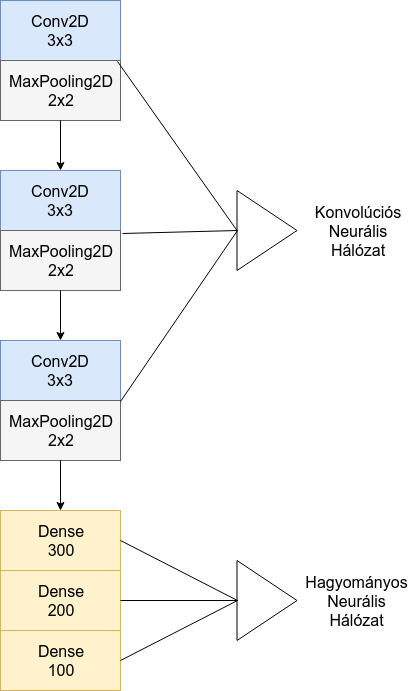
\includegraphics[scale=0.45]{images/cnn_architecture}
\caption{Architektúra}
\label{fig:cnn_arch}
\end{figure}

Az első konvolúciós réteg a nyers képet bevitelként veszi fel, majd a különböző dimenzió mentén működő neuronok aktiválódhatnak különböző orientált élek vagy színes foltok jelenlétében.

A pooling réteg a kép térbeli méretének fokozatos csökkentésére, a paraméterek számának és a számítás számának csökkentésére szolgál a hálózatban. Továbbá kontrollálja a túltanítás jelenséget.

Fontos megjegyezni, hogy a szűrők az eredeti bemeneti kép jellemződetektoraként működnek.

A szűrőmátrix (filter) különböző értékei ugyanazon bemeneti képhez különböző jellemző-térképeket eredményeznek. Példaként vegye figyelembe néhány szűröt, amely képes felismerni a különböző jellemzőket:
\begin{itemize}
\item Él detektálás: 
$
\begin{bmatrix}
\ \ 1 & 0 & -1 \\
\ \ 0 & 0 & \ \ 0 \\
-1 & 0 & \ \ 1
\end{bmatrix}
$
$
\begin{bmatrix}
0 &  \ \ 1 & 0 \\
1 & -4 & 1 \\
0 &  \ \ 1 & 0
\end{bmatrix}
$
$
\begin{bmatrix}
-1 &  -1 & -1 \\
-1 & \ \ 8 & -1 \\
-1 &  -1 & -1
\end{bmatrix}
$
\item Élesség: $\begin{bmatrix}
\ \ 0 & -1 & \ \ 0 \\
-1 & \ \ 5 & -1 \\
\ \ 0 & -1 & \ \ 0
\end{bmatrix}$
\item Elmosodás (Gaussian blur): $\frac{1}{16}
\begin{bmatrix}
1 & 2 & 1 \\
2 & 4 & 2 \\
1 & 2 & 1
\end{bmatrix}$
\end{itemize}

Az előterjesztésbe (forward pass) a pixelek értékei áthaladnak a konvolúciós rétegeken, amelyek kiszámítják a mátrixok (szűrő és pixel mátrix) szorzatát. A manipulált pixel értékeket a hálózat továbbadja a következő rétegnek és a különböző jellemző térképét. Ennek eredményeképpen a hálózat megtanulja a szűrőket, amelyek akkor aktiválódnak, amikor valamilyen konkrét típusú jellemzőt észlelnek bizonyos térbeli pozícióban a bemenetben.
